\documentclass[12pt]{article}
\usepackage[utf8]{inputenc}
\usepackage{graphicx} % Allows you to insert figures
\usepackage{amsmath} % Allows you to do equations
\usepackage{fancyhdr} % Formats the header
\usepackage{geometry} % Formats the paper size, orientation, and margins
\linespread{1.25} % about 1.5 spacing in Word
\setlength{\parindent}{0pt} % no paragraph indents
\setlength{\parskip}{1em} % paragraphs separated by one line
\usepackage[format=plain,
            font=it]{caption} % Italicizes figure captions
\usepackage[english]{babel}
\usepackage{csquotes}
\renewcommand{\headrulewidth}{0pt}
\geometry{letterpaper, portrait, margin=1in}
\setlength{\headheight}{14.49998pt}

\newcommand\titleofdoc{\textbf{Assignment-3: Fitting Data to Models}}
\newcommand\GroupName{EE20B136}

\begin{document}
\begin{titlepage}
   \begin{center}
        \vspace*{4cm} % Adjust spacings to ensure the title page is generally filled with text

        \Huge{\titleofdoc} 

        \vspace{3 cm}
        \Large{Syam SriBalaji T}
       
        \vspace{0.25cm}
        \large{EE20B136}
       
        \vspace{3 cm}
        \Large{February 18, 2022}
        
        \vspace{0.25 cm}
        \Large{EE2703 :Jan-May 2022}
       

       \vfill
    \end{center}
\end{titlepage}

\setcounter{page}{2}
\pagestyle{fancy}
\fancyhf{}
\rhead{\thepage}

\section*{Question:4}

True value graph mentioned here is found by: g(t;A,B) = A*J2 (t) +B*t ,where A=1.05,B=-0.105 \linebreak 
The other plots are Data of each column vs. Time

\begin{figure}[h!]
\centering
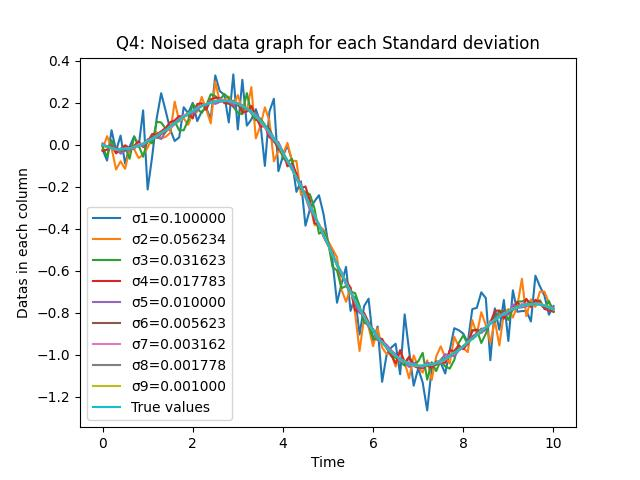
\includegraphics[height=15cm]{Figure_2.jpeg}
\end{figure}

\newpage
\section*{Question:5}

Plot for the first column of data with error bars and also only every 'Fifth' data item is plotted here to make the plot readable. And the True value graph is also plotted to see the divergence in error bar.

\begin{figure}[h!]
\centering
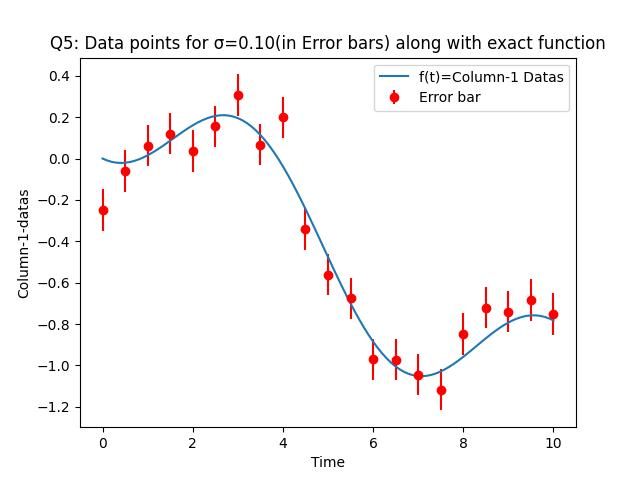
\includegraphics[height=15cm]{Figure_3.jpeg}
\label{fig:exemplo}
\end{figure}

\newpage
\section*{Question:8}

Plotting of the contour graph using the Mean squared matrix found (of Column 1 data).
\linebreak
Yes, it has minimum (single).

\begin{figure}[h!]
\centering
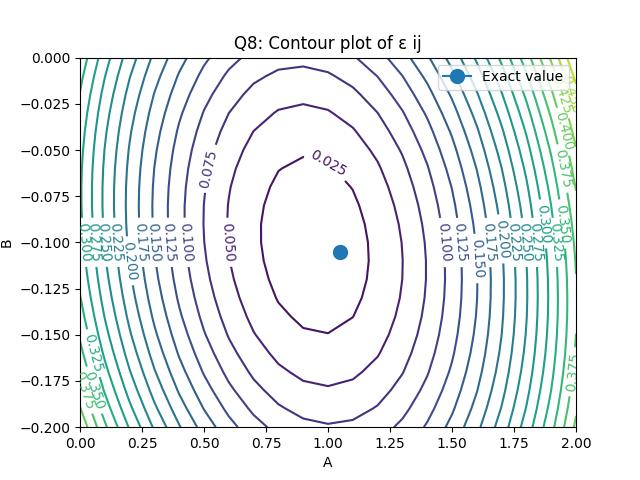
\includegraphics[height=15cm]{Figure_4.jpeg}
\end{figure}

\newpage
\section*{Question:10}

Creating different sets of noised datas and finding graph of errors in estimation of A \& B.\linebreak
\linebreak
Yes, Both Error for A \& B increases with increase in Standard deviation, while A increases more drastically than B.

\begin{figure}[h!]
\centering
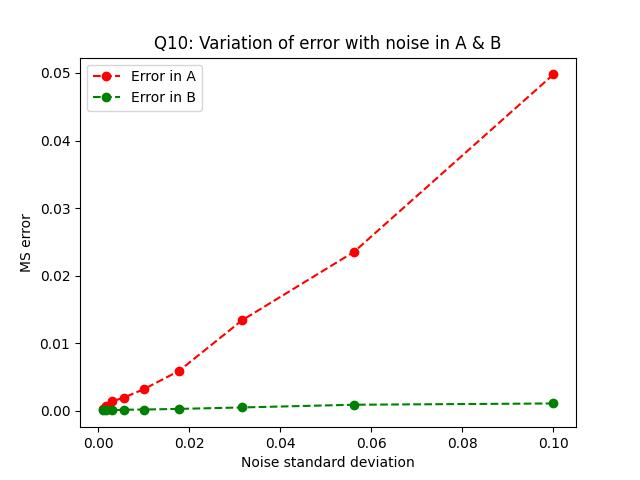
\includegraphics[height=15cm]{Figure_5.jpeg}
\end{figure}

\newpage
\section*{Question:11}

Plotting the same Errors of A \& B as in previous question but with the help of loglog() function
\linebreak
We can notice the increase in Error values wrt to Standard deviation clearly here.

\begin{figure}[h!]
\centering
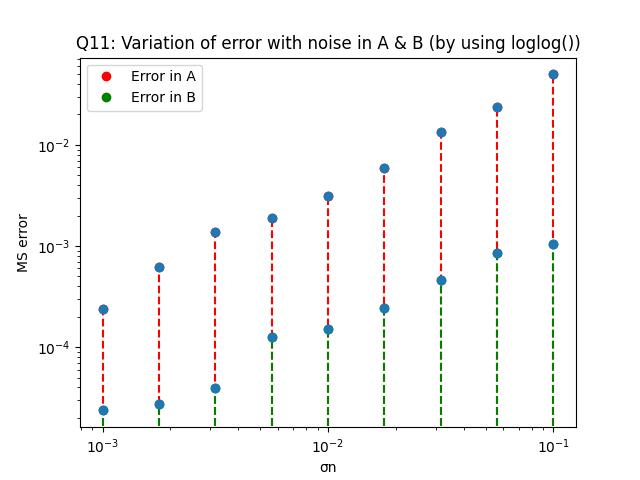
\includegraphics[height=15cm]{Figure_6.jpeg}
\end{figure}

\end{document}
